\documentclass{article}

\usepackage{amsmath}
\usepackage{amssymb}
\usepackage{bm}
\usepackage{graphicx}
\usepackage{epstopdf}
\DeclareGraphicsRule{.tif}{png}{.png}{`convert #1 `basename #1 .tif`.png}
\usepackage{color}
\usepackage{pdfsync}
\pagestyle{plain}

\textheight 9 true in
\textwidth 6.5 true in
\hoffset -.75 true in
\voffset -.75 true in
\mathsurround=2pt
\parskip=2pt

\begin{document}

\begin{center}
\large{ MATH-2400 \hspace{.27in}  INTRODUCTION TO DIFFERENTIAL EQUATIONS \hspace{.27in}FALL 2022\bigskip\\ {\bf Problem Set 10} \smallskip\\ Due: 11pm, Tuesday, December 6, 2022}
\\Hayden Fuller
\end{center}

\bigskip\noindent
\underline{NOTES}
\begin{enumerate}
\item Practice problems listed below and taken from the textbook are for your own practice, and are not to be turned in.
\item There are two parts of the Problem Set, an objective part consisting of multiple choice questions (with no partial credit available) and a subjective part (with partial credit possible).  Please complete all questions.
\item Writing your solutions in {\LaTeX} is preferred but not required.
\item Show all work for problems in the subjective part.  Illegible or undecipherable solutions will not be graded. 
\item Figures, if any, should be neatly drawn by hand, properly labelled and captioned.  
\item Your completed work is to be submitted electronically to LMS  as a \textcolor{red}{single pdf file}. Be sure that the pages are properly oriented and well lighted.  (\textcolor{blue}{Please do not e-mail your work to Muhammad or me.})
\end{enumerate}

\bigskip\noindent
{\bf Practice Problems from the textbook} (Not to be turned in)
\begin{itemize}
\item
Exercises from Chapter 4, pages 83--84: 1(d,e), 2(b), 3(c,d).
\item
Exercises from Chapter 4, page 91: 1(a,b), 2(a,b).
\item
Exercises from Chapter 4, page 98: 1(a,c), 2(a,c).
\item
Exercises from Chapter 4, page 105--107: 2(a,b), 3(a,b).
\end{itemize}

\bigskip\noindent
{\bf Objective part} (Choose A, B, C or D; no work need be shown, no partial credit available)

\begin{enumerate}
\item (5 points) Let
\[
A=\begin{bmatrix}\;\;1&2&\alpha\smallskip\\ -4&1&2\smallskip\\ -1&\beta&1\end{bmatrix}
\]
where $\alpha$ and $\beta$ are constants.  Which statement is true or select ``All of these choices'' if all statements are true:
\begin{description}
\item[A]  $A$ is singular if $\alpha=\beta=1$
\item[B]  $A$ is nonsingular if $\alpha=0$ and $\beta=2$
\item[C]  The column vectors of $A$ are linearly dependent if $\alpha=-1$ and $\beta=-2$
\item[D]  X All of these choices. X
\end{description}

\bigskip
\item (5 points)  Let ${\bf x}(t)$ solve the constant-coefficient system
\[
{\bf x}\sp\prime=A{\bf x},\qquad A=\begin{bmatrix}1&1\\ 4&3\end{bmatrix}
\]
Which statement is true or select ``None of these choices'' if none of the statements are true:
\begin{description}
\item[A] The phase portrait of the system is a source.
\item[B] X The phase portrait of the system is a saddle. X
\item[C] The phase portrait of the system is a sink.
\item[D] None of these choices.
\end{description}

\bigskip
\item (5 points) Let ${\bf x}(t)$ solve the constant-coefficient system
\[
{\bf x}\sp\prime=A{\bf x},\qquad A=\begin{bmatrix}\;3&\;\;5\;\\ \;a&-3\;\end{bmatrix}
\]
The phase portrait of the system is a center if
\begin{description}
\item[A]  $a=0$
\item[B]  $a=-1$
\item[C]  X $a=-2$ X
\item[D]  None of these choices.
\end{description}


\end{enumerate}

\bigskip\bigskip\noindent
{\bf Subjective part} (Show work, partial credit available)

\begin{enumerate}

\item (15 points)  Let ${\bf x}(t)$ satisfy the initial-value problem
\[{\bf x}^\prime=\left[\begin{array}{cc}1&-2 \smallskip\\3&-4\end{array}\right]{\bf x},\qquad{\bf x}(0)=\left[\begin{array}{c}-2 \smallskip\\-1\end{array}\right]\]
\begin{enumerate}
\item
Find the general solution of the constant-coefficient system.
\\$p(r)=r^2+3r+2=(r+2)(r+1)$
\\$r_1=-2$, $r_2=-1$
\\$(A-r_1I)z_1=0=\left[\begin{array}{cc}3&-2 \smallskip\\3&-2\end{array}\right]z_1$; $z_1=[a\;\;b]^T$; $3a-2b=0$; $3a=2b$; $1.5a=b$;  $z_1=[2\;\;3]^T$
\\$(A-r_2I)z_2=0=\left[\begin{array}{cc}2&-2 \smallskip\\3&-3\end{array}\right]z_2$; $z_2=[a\;\;b]^T$; $a-b=0$; $a=b$; $z_2=[1\;\;1]^T$
\\$x(t)=C_1[2\;\;3]^Te^{-2t}+C_2[1\;\;1]^Te^{-t}$
\item
Find the solution of the initial-value problem.
\\$x(0)=[-2\;\;-1]^T=C_1[2\;\;3]^Te^{0}+C_2[1\;\;1]^Te^{0}=C_1[2\;\;3]^T+C_2[1\;\;1]^T$; $C_1=1$; $C_2=-4$
\\$x(t)=[2\;\;3]^Te^{-2t}-4[1\;\;1]^Te^{-t}$
\end{enumerate}




\bigskip
\item (15 points)  Consider the two systems of first-order ODEs:
\[\hbox{(a)}\quad\begin{array}{l}x_1\sp\prime=2x_1+2x_2\smallskip\\x_2\sp\prime=\;\;x_1+3x_2\end{array}\qquad\qquad\qquad
\hbox{(b)}\quad\begin{array}{l}x_1\sp\prime=x_1+5x_2\smallskip\\x_2\sp\prime=x_1-3x_2\end{array}
\]
Determine the general solution for ${\bf x}(t)=[x_1(t)\,,\,x_2(t)]\sp{T}$ for each system and plot their phase portraits.  Classify the solution behavior as to its type (e.g.~saddle, source, etc.).  Note: be sure to plot lines parallel to the eigenvectors for each phase portrait and sketch representative trajectories for increasing $t$ in the four regions separated by the lines parallel to the eigenvectors.
\\a)
\\$x'=\left[\begin{array}{cc}2&2 \smallskip\\1&3\end{array}\right]x$
\\$p(r)=r^2-5r+4=(r-4)(r-1)$
\\$r_1=1$; $r_2=4$
\\$(A-r_1I)z_1=0=\left[\begin{array}{cc}1&2 \smallskip\\1&2\end{array}\right]z_1$; $z_1=[a\;\;b]^T$; $a+2b=0$; $a=-2b$; $z_1=[-2\;\;1]^T$
\\$(A-r_2I)z_2=0=\left[\begin{array}{cc}-2&2 \smallskip\\1&-1\end{array}\right]z_2$; $z_2=[a\;\;b]^T$; $a-b=0$; $a=b$; $z_2=[1\;\;1]^T$
\\$x(t)=C_1[-2\;\;1]^Te^{t}+C_2[1\;\;1]^Te^{4t}$
\\Source
\begin{figure}[h]
\centerline{\fbox{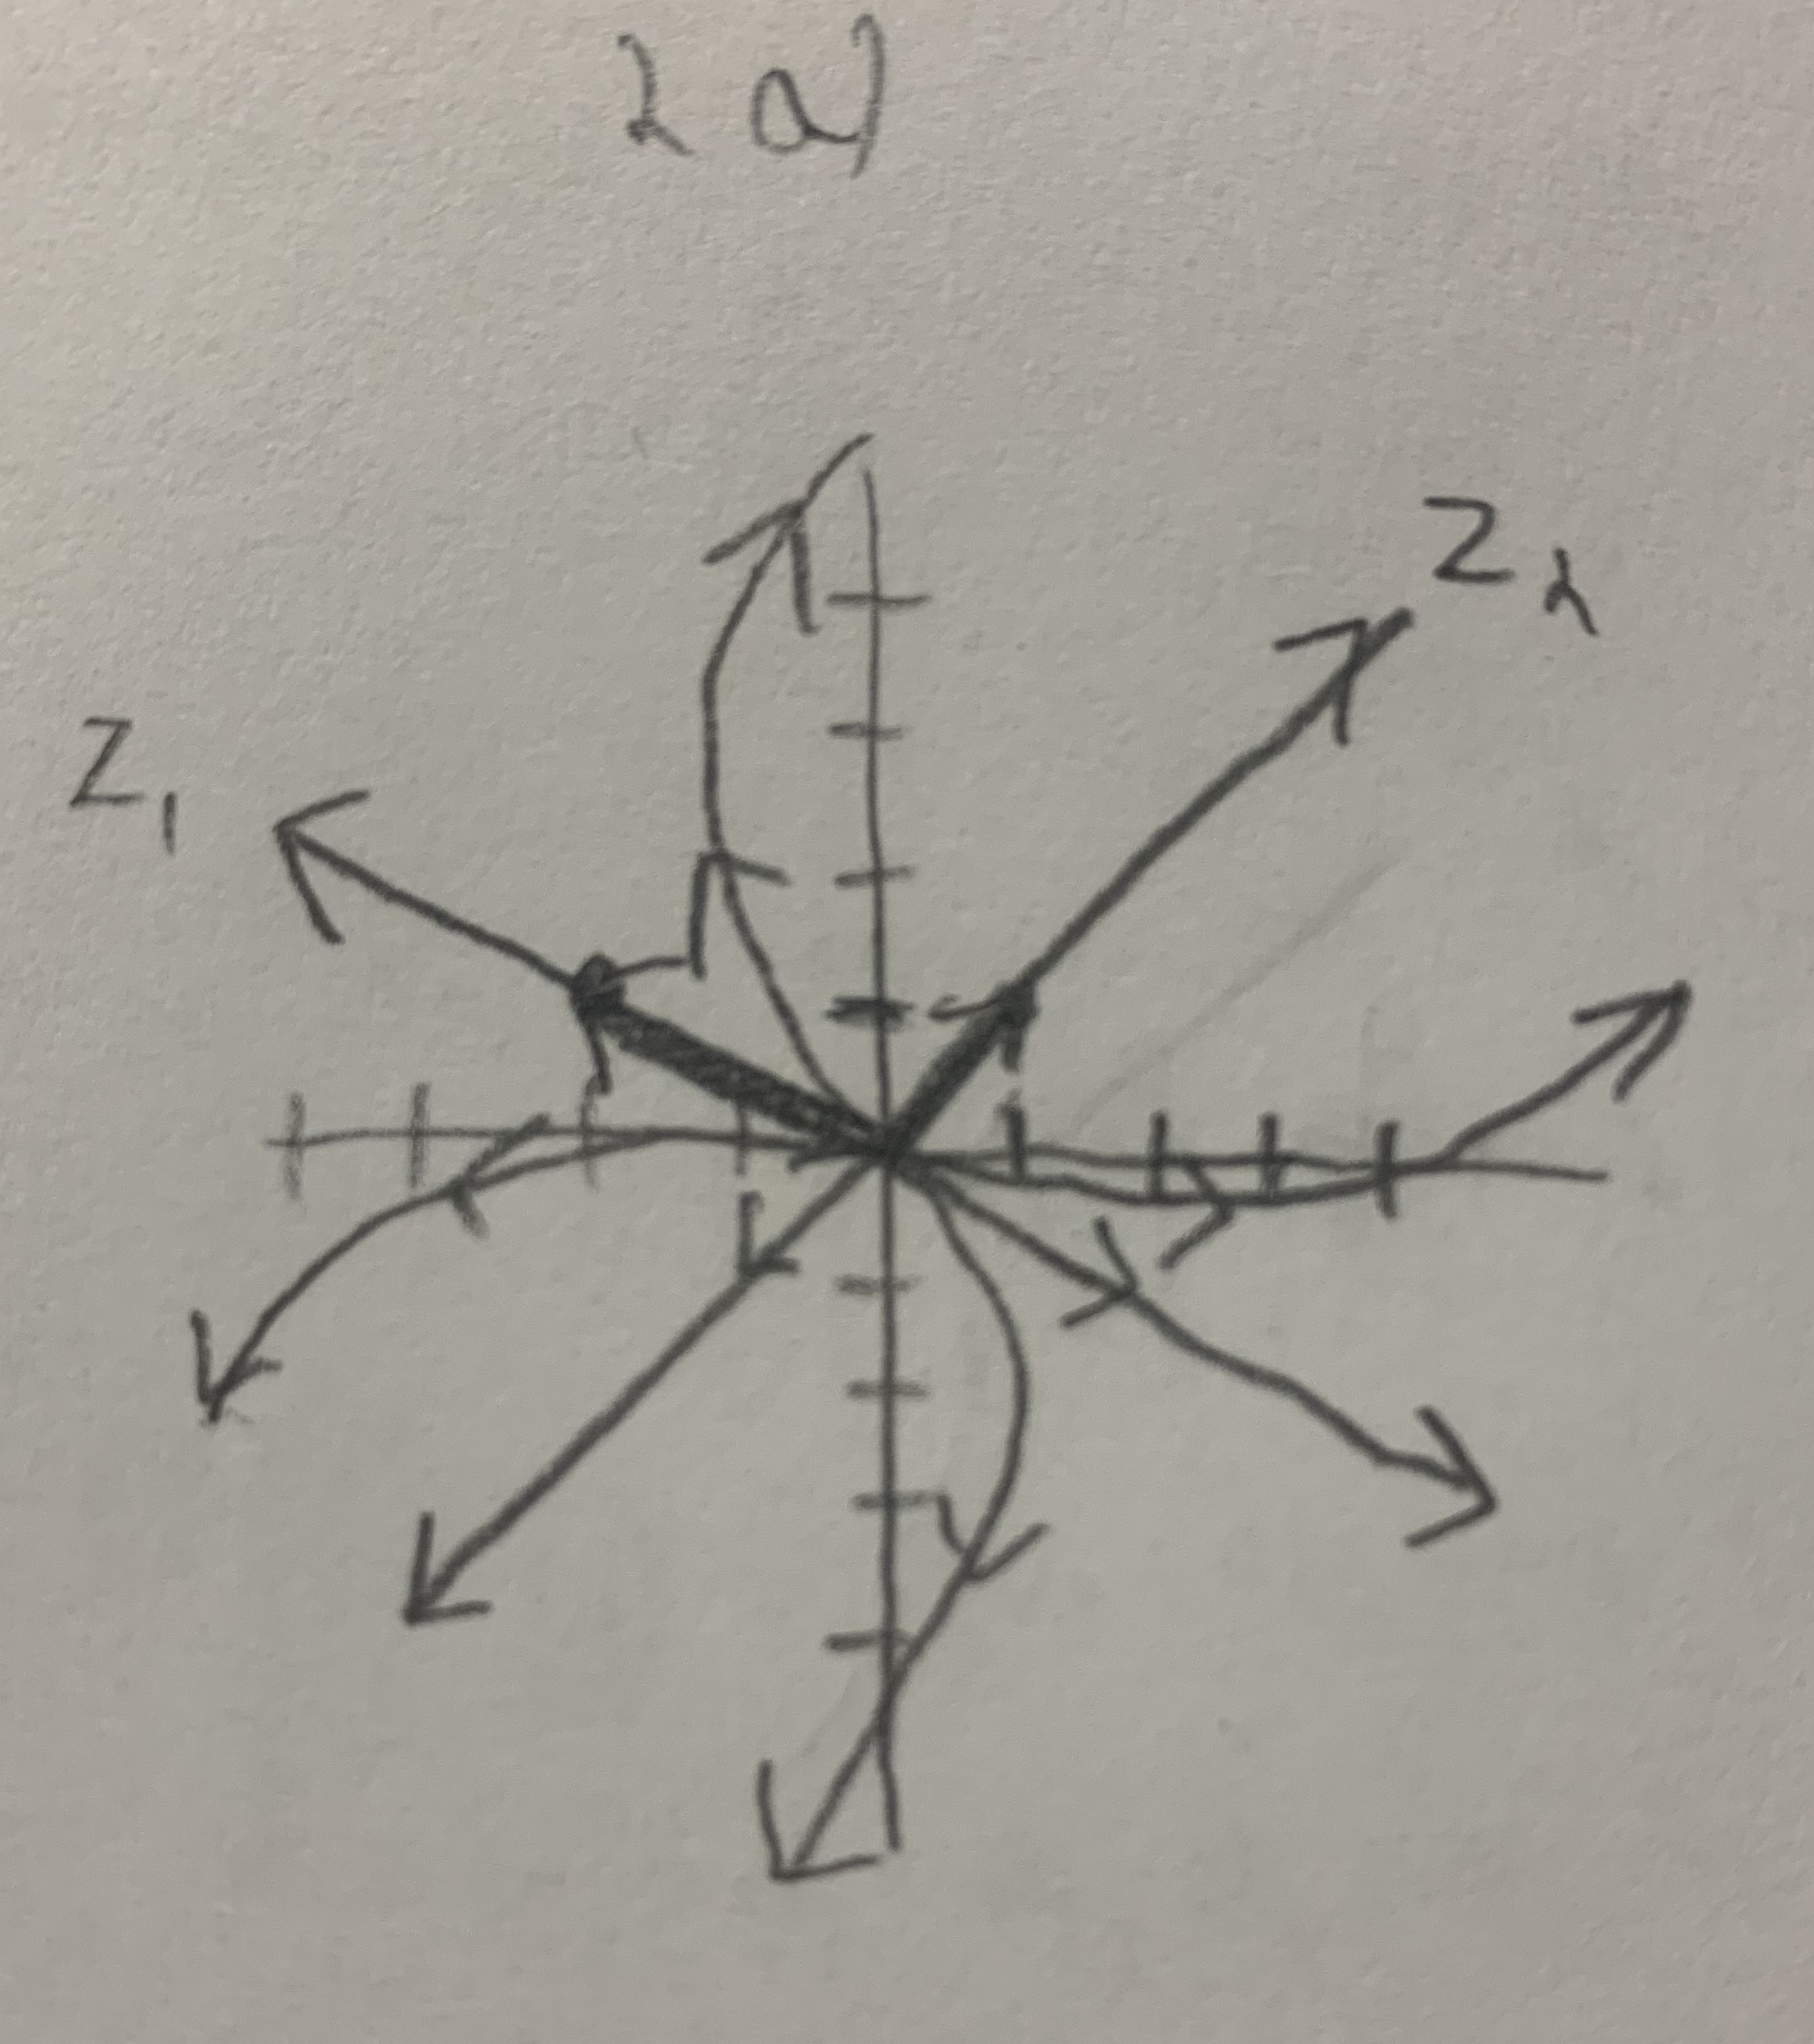
\includegraphics[scale=0.1]{PS10S2A}}}
\end{figure}
\\
\\b)
\\$x'=\left[\begin{array}{cc}1&5 \smallskip\\1&-3\end{array}\right]x$
\\$p(r)=r^2+2r-8=(r-2)(r+4)$
\\$r_1=2$; $r_2=-4$
\\$(A-r_1I)z_1=0=\left[\begin{array}{cc}-1&5 \smallskip\\1&-5\end{array}\right]z_1$; $z_1=[a\;\;b]^T$; $a-5b=0$; $a=5b$; $z_1=[5\;\;1]^T$
\\$(A-r_2I)z_2=0=\left[\begin{array}{cc}5&5 \smallskip\\1&1\end{array}\right]z_2$; $z_2=[a\;\;b]^T$; $a+b=0$; $a=-b$; $z_2=[1\;\;-1]^T$
\\$x(t)=C_1[5\;\;1]^Te^{2t}+C_2[1\;\;-1]^Te^{-4t}$
\\Saddle
\begin{figure}[h]
\centerline{\fbox{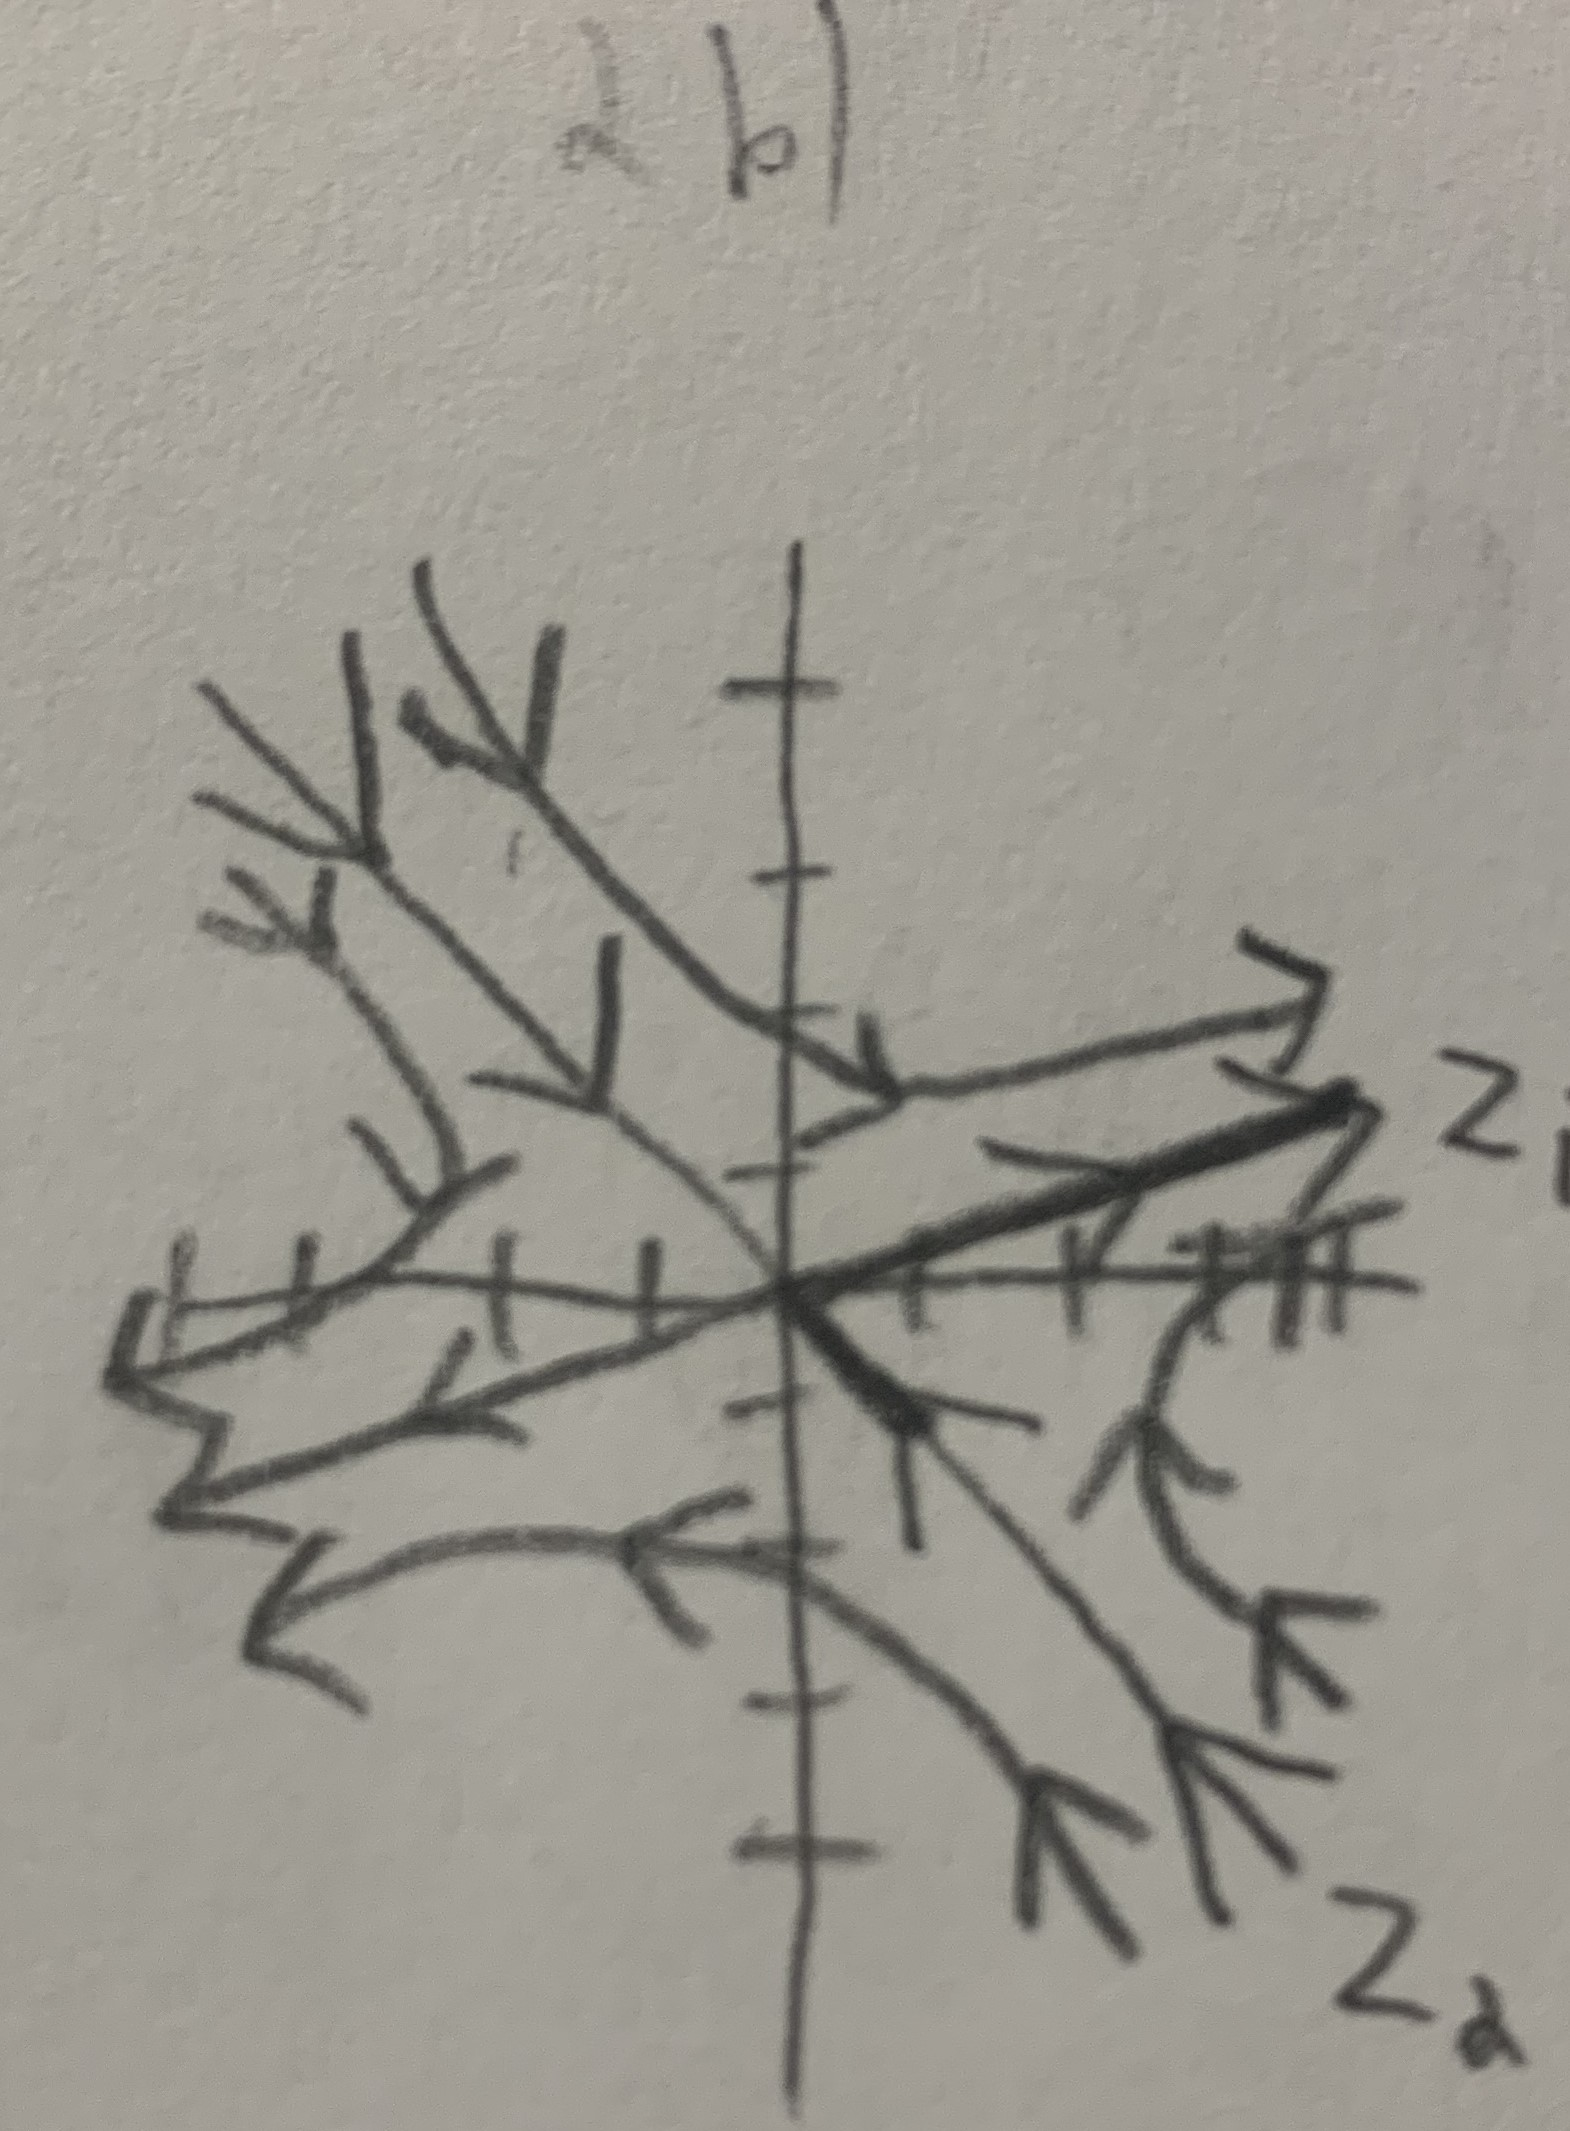
\includegraphics[scale=0.1]{PS10S2B}}}
\end{figure}
\newpage




\bigskip
\item (15 points) Consider the constant-coefficient system
\[
{\bf x}\sp\prime=A{\bf x},\qquad
A=\left[
\begin{array}{rr}
3&-2\smallskip\\
4&-1
\end{array}
\right]
\]
\begin{enumerate}
\item
Find the eigenvalues and eigenvectors of $A$.
\\$p(r)=r^2-2r+5$
\\$r=\frac{2\pm\sqrt{4-20}}{2}=1\pm2i$
\\$r_1=1+2i$; $r_2=1-2i$
\\$A-r_1I=\left[
\begin{array}{rr}2-2i&-2\smallskip\\4&-2-2i\end{array}\right]$; $A-r_2I=\left[\begin{array}{rr}2+2i&-2\smallskip\\4&-2+2i\end{array}\right]$
\\$\left[\begin{array}{rr}2-2i&-2\smallskip\\4&-2-2i\end{array}\right]z=0$
\\$\left[\begin{array}{rr}-1+i&1\smallskip\\-2&1+i\end{array}\right]z=0$
\\$z_1=\left[\begin{array}{rr}1\smallskip\\1-i\end{array}\right]=\left[\begin{array}{rr}1+i\smallskip\\2\end{array}\right]$; $z_2=\left[\begin{array}{rr}1\smallskip\\1+i\end{array}\right]$
\item
Find the general solution of the system in terms of real-valued functions.
\\$x_1=(a+ib)e^{(\lambda+i\mu)t}$; $a=[1\;\;1]^T$; $b=[0\;\;1]^T$; $\lambda=1$; $\mu=2$
\\$u(t)=(a\cos(2t)-b\sin(2t))e^t=([1\;\;1]^T\cos(2t)-[0\;\;1]^T\sin(2t))e^t$
\\$v(t)=(b\cos(2t)+a\sin(2t))e^t=([0\;\;1]^T\cos(2t)+[1\;\;1]^T\sin(2t))e^t$
\item
Sketch the phase portrait for the system and classify the solution behavior as to its type (e.g.~saddle, source, etc.)  Note: when the eigenvalues and eigenvectors are complex conjugates, it is helpful to plot lines parallel to the real and imaginary parts of the eigenvectors.
\\Spiral Source
\begin{figure}[h]
\centerline{\fbox{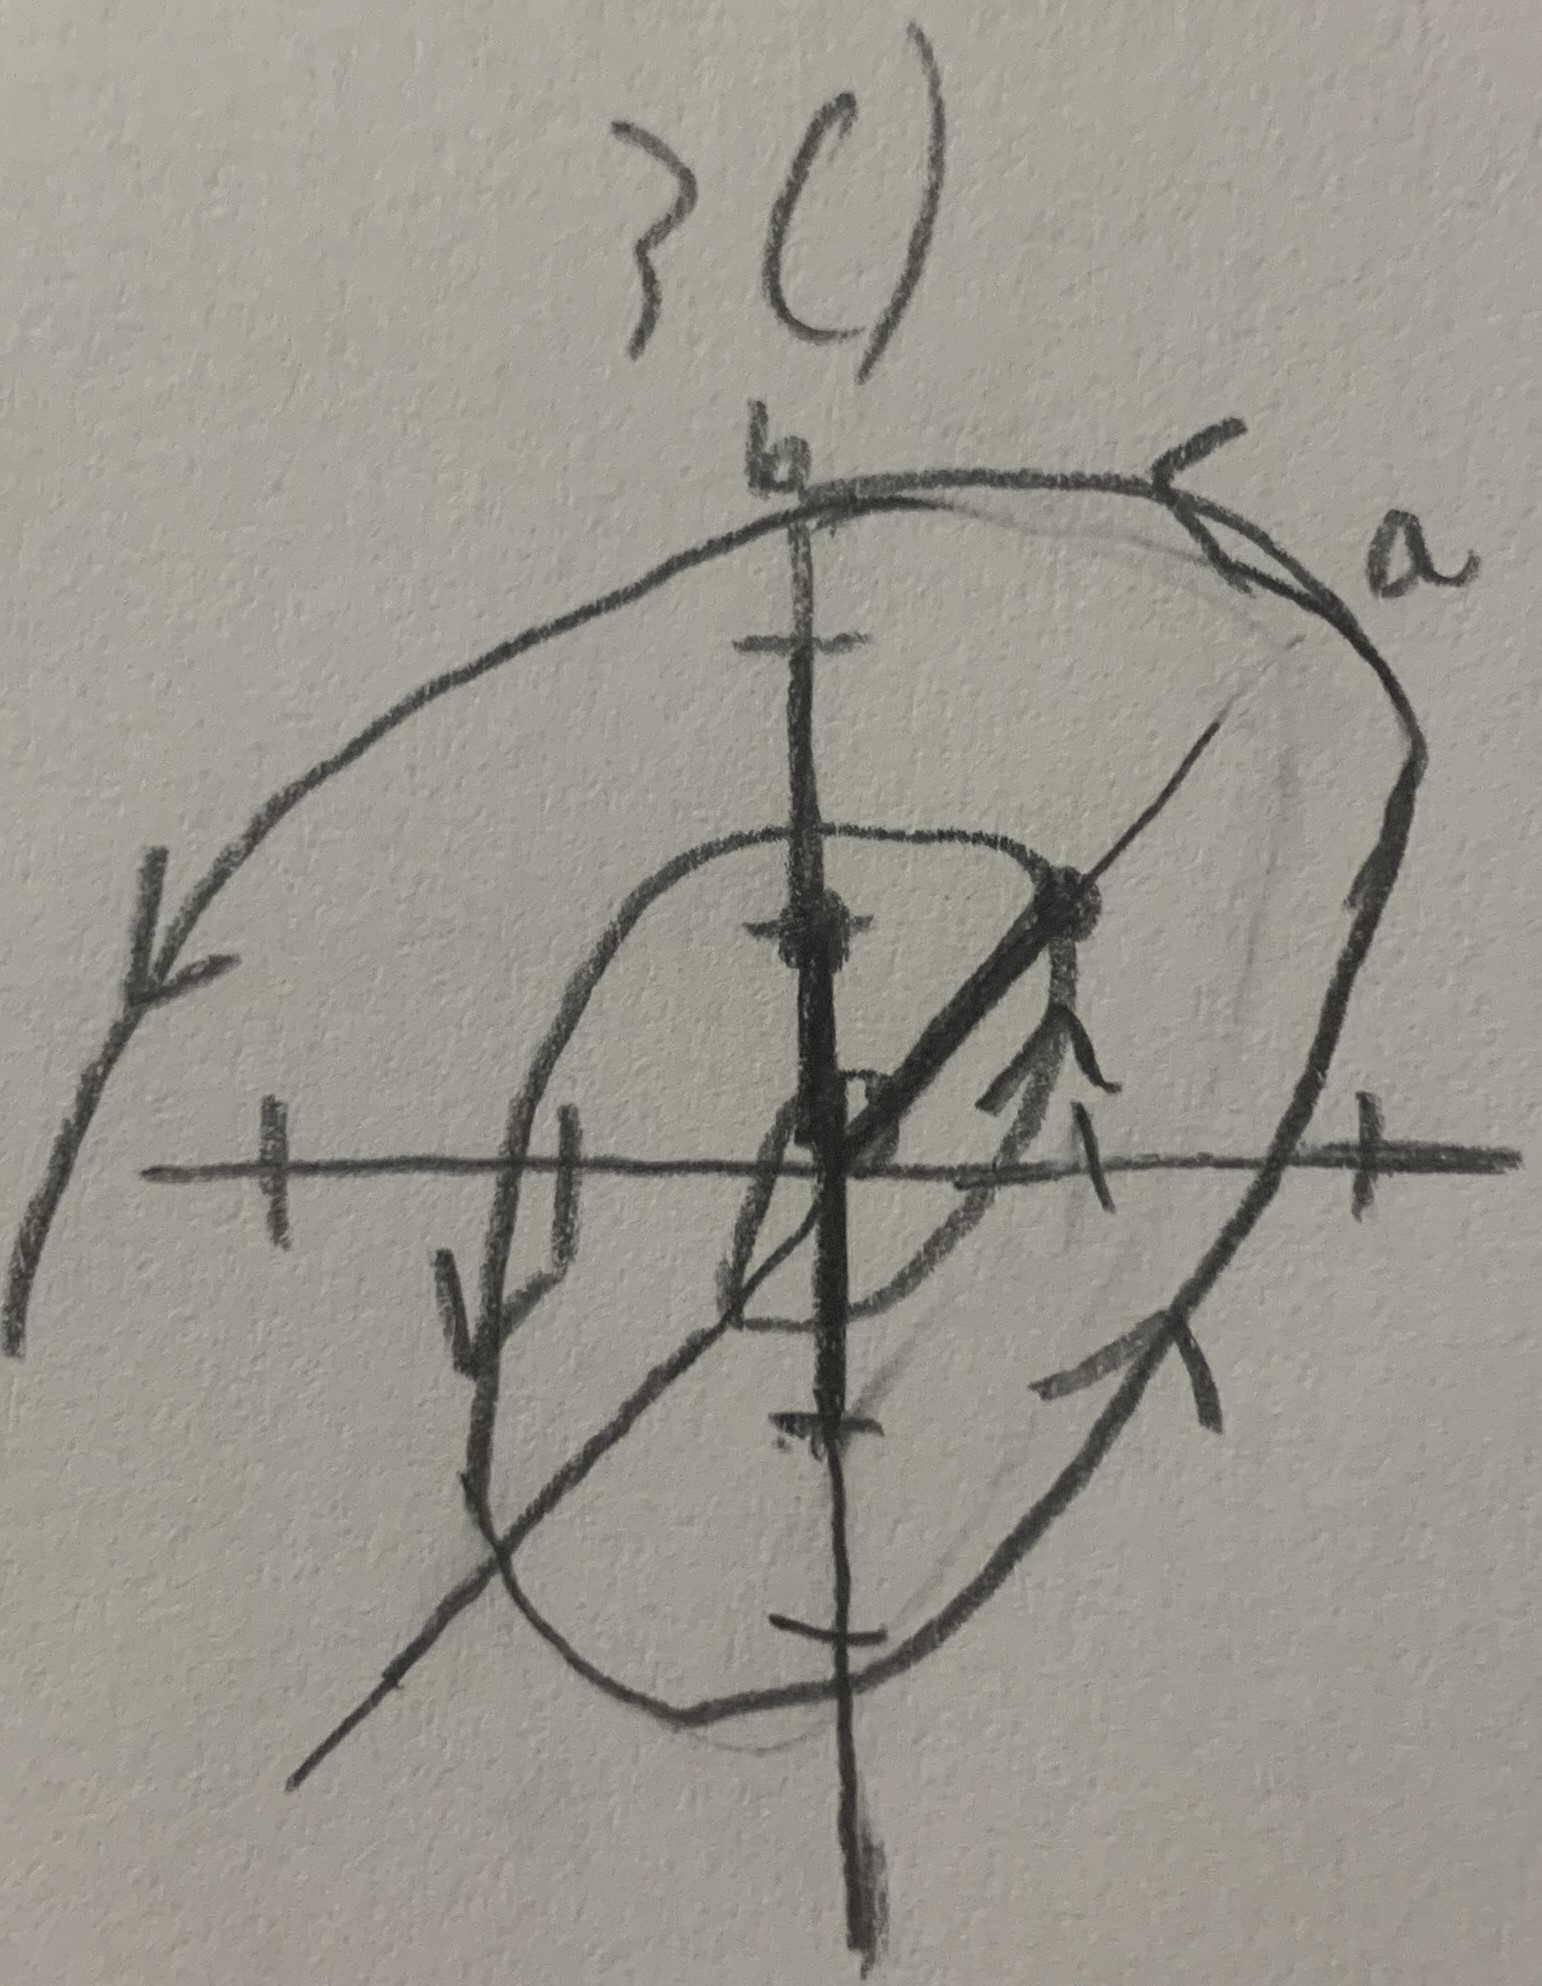
\includegraphics[scale=0.1]{PS10S3Ccc}}}
\end{figure}
\end{enumerate}





\end{enumerate}



\end{document}



























